% use no footline.
\begin{frame}[plain, noframenumbering]{Outline}
	\tableofcontents
\end{frame}
%%%%%%%%%%%%%%%%%%%%%%%%%%%%%%%%%%%%%%%%%%%%%%%%%%%%%%
\section{Hive}



\begin{frame}
\frametitle{Chapter Objectives}

\begin{itemize}
	\item<1-> Query data lakes/HDFS using Hive. \pause
	\item<2-> Introduction to Hive \pause
	\item<3-> Comparing Hive to Traditional databases.
	\item<4-> Hive Components and Architecture. \pause
	\item<5-> Relational Data Analysis with Hive. \pause
	\item<6-> Hive Data Management. \pause
	\item<7-> Hive Optimization. \pause
\end{itemize}

\end{frame}

%%%%%%%%%%%%%%%%%%%%%%%%%%%%%%%%%%%%%%%%%%%%%%%%%%%%%%
\subsection{Query data lakes/HDFS using Hive}
\begin{frame}
	\frametitle{\subsecname}
	\begin{itemize} 
		\item Data lakes and HDFS store vast amounts of petabyte-scale data. \pause
		\item Data analysts require efficient ways to query this data without delving into intricate Map-Reduce programming.\pause
		\item SQL is a commonly used language for data manipulation, embraced by data analysts, developers, and business users worldwide.\pause
		\item Hive, one of the early tools in this field, simplifies data analysis on big data by offering SQL-like querying capabilities for data lakes and HDFS.\pause
		\item There are other tools like Trino/Presto, Snowflake, and Databricks that can be faster for data lake queries, which we will discuss later.\pause
	\end{itemize}
	\end{frame}
%%%%%%%%%%%%%%%%%%%%%%%%%%%%%%%%%%%%%%%%%%%%%%%%%%%%%%

\subsection{Introduction to hive}
\begin{frame}
\frametitle{\subsecname}
\begin{itemize} 
	\item Apache Hive is a powerful data warehousing and SQL-like query language tool within the Hadoop ecosystem.\pause
	\item It was developed by Facebook and later contributed to the Apache Software Foundation, making it an open-source project.\pause
	\item Apache Hive had its initial release on October 1, 2010.	\pause
\end{itemize}
\end{frame}

\begin{frame}
	\frametitle{\subsecname}
	\begin{itemize} 
		\item Hive provides a user-friendly interface to work with and analyze large datasets stored in Hadoop Distributed File System (HDFS) or other compatible storage systems.\pause
		\item With its SQL-like language called HiveQL, users can write queries to extract, transform, and analyze data, making it accessible to a wide range of data professionals\pause
		\item Apache Hive bridges the gap between the world of big data and traditional relational databases, making it a valuable tool for data engineers, analysts, and data scientists.\pause	
	\end{itemize}
	\end{frame}
%%%%%%%%%%%%%%%%%%%%%%%%%%%%%%%%%%%%%%%%%%%%%%%%%%%%%%


\subsubsection{Overview of Apache Hive}
\begin{frame}
\frametitle{Overview of Apache Hive}
\begin{itemize} 
	\item Apache Hive is a high-level data warehousing and SQL-like query language tool built on top of MapReduce.\pause
	\item It acts as an abstraction layer, allowing users to work with large datasets stored in Hadoop Distributed File System (HDFS) without needing to write complex MapReduce jobs themselves.\pause
	\item Under the hood, Hive generates MapReduce jobs that are executed on the Hadoop cluster. This means it leverages the distributed processing capabilities of Hadoop for scalability and parallel processing.\pause
	\item Hive has evolved beyond MapReduce to support other execution engines, such as Tez and Spark, which can enhance performance and usability. This will be discussed later.\pause

\end{itemize}
\end{frame}

%%%%%%%%%%%%%%%%%%%%%%%%%%%%%%%%%%%%%%%%%%%%%%%%%%%%%%

\subsection{Hive Architecture}

\begin{frame}{Abstract Components of Apache Hive}
	\begin{itemize}
		\item Hive Clients.
		\item Hive Services.
		\item Hive Storage and Computing.
	\end{itemize}
	\end{frame}
	
\begin{frame}{Abstract Components of Apache Hive}
	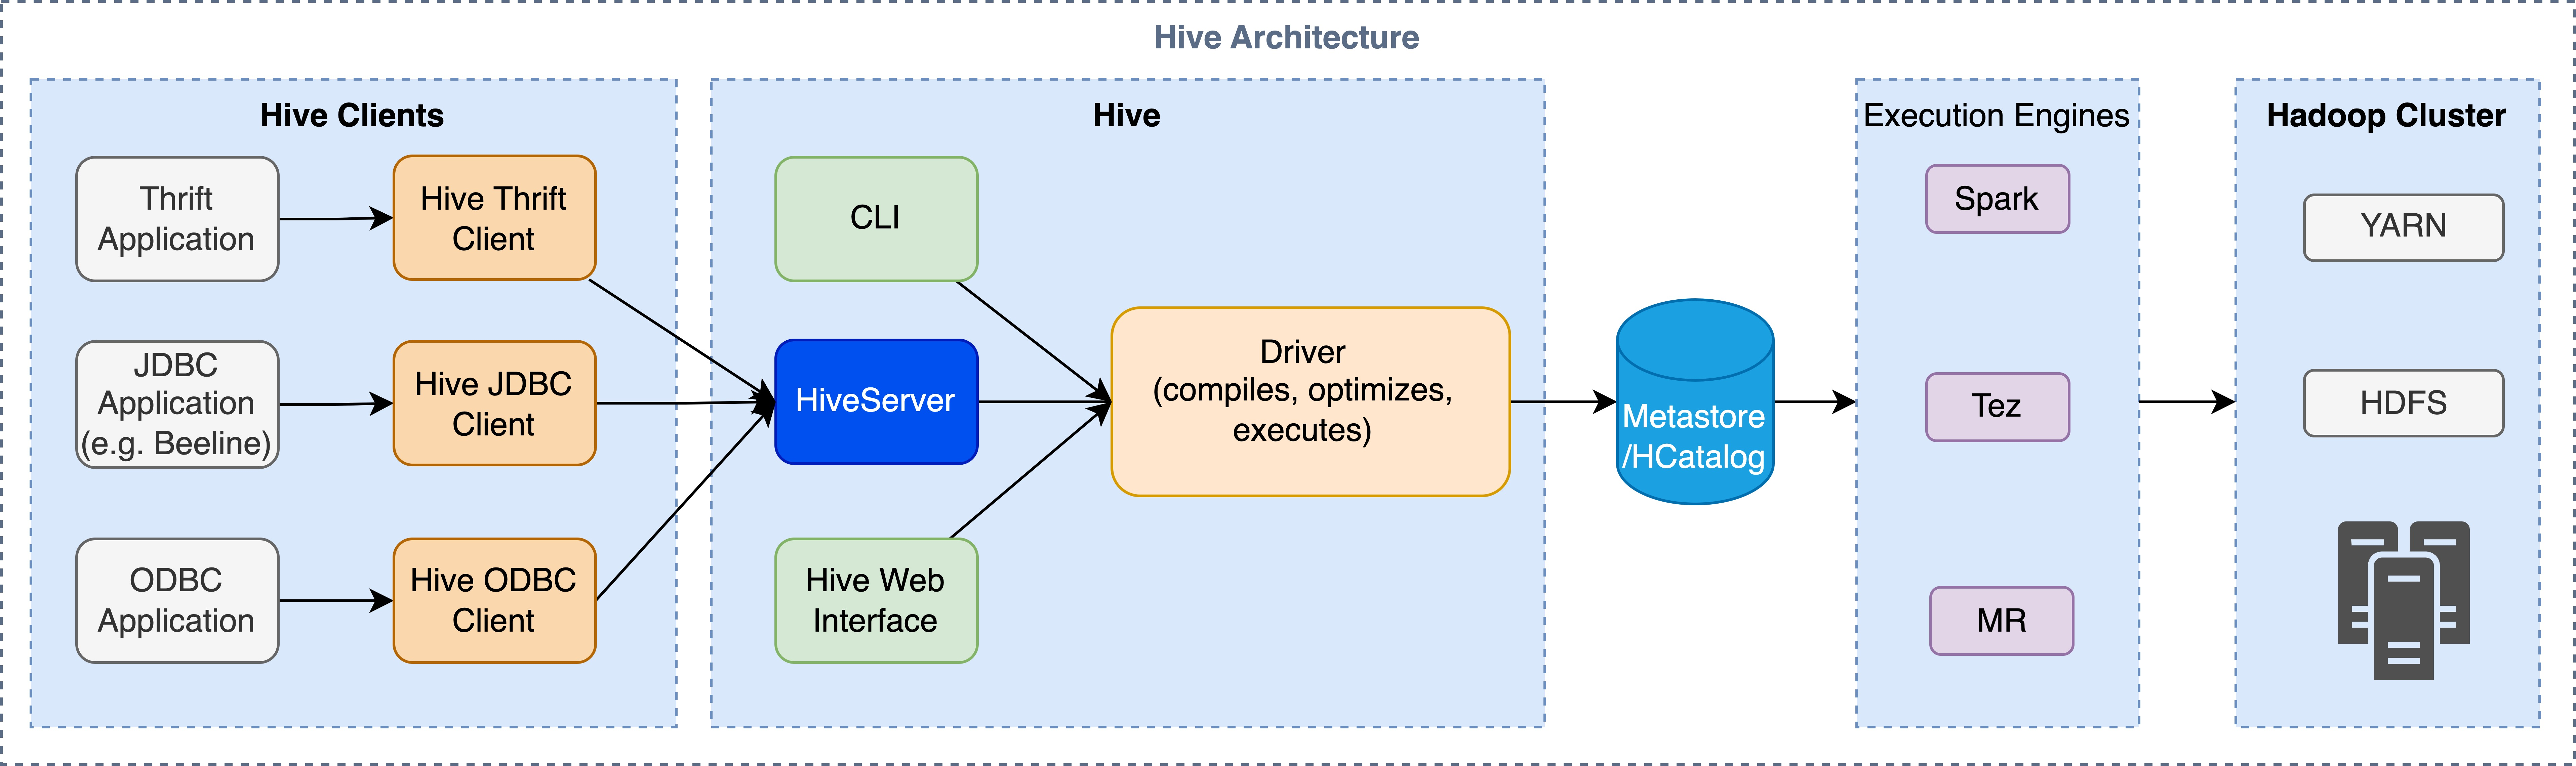
\includegraphics[width=\linewidth,height=.8\textheight]{./Figures/chapter-03/Hive_Architecture.jpg}
\end{frame}
	

%%%%%%%%%%%%%%%%%%%%%%%%%%%%%%%%%%%%%%%%%%%%%%%%%%%%%%
\begin{frame}
\frametitle{Hive Clients}
	\framesubtitle{Connecting with Hive}
	
	\begin{itemize}
	  \item Hive provides various drivers for seamless communication with different types of applications.
	  \item For Thrift-based applications, Hive offers the Thrift client for effective communication.
	  \item If you are working with Java-related applications, Hive provides JDBC drivers for smooth integration.
	  \item Additionally, for other types of applications, Hive offers ODBC drivers, ensuring versatility.
	  \item These clients and drivers serve as intermediaries, connecting your applications with Hive Server in the Hive services.
	\end{itemize}
	
	\end{frame}
%%%%%%%%%%%%%%%%%%%%%%%%%%%%%%%%%%%%%%%%%%%%%%%%%%%%%%
\begin{frame}
	\frametitle{Hive Services}
	\framesubtitle{Client Interactions}
	
	\begin{itemize}
	  \item Hive Services act as the intermediaries for client interactions with Hive.
	  \item When clients need to perform query-related operations in Hive, they communicate through Hive Services.
	  %\item The Command Line Interface (CLI) serves as a Hive service for Data Definition Language (DDL) operations.
	  \item All drivers, including JDBC, ODBC, and other client-specific applications, communicate with Hive Server and the primary driver within Hive Services.
	  \item The main driver in Hive Services processes requests from various applications, directing them to the metastore and data systems for further processing.
	\end{itemize}
	
	\end{frame}
%%%%%%%%%%%%%%%%%%%%%%%%%%%%%%%%%%%%%%%%%%%%%%%%%%%%%%

	\begin{frame}
		\frametitle{Hive Services | CLI (Continued)}
		\framesubtitle{Hive CLI Challenges}
		
		\begin{itemize}
		  \item Hive Command Line Interface (CLI)
		  	\begin{itemize}
				\item  The CLI is the most common way to access Hive.
				\item  Its design can make it challenging to use programmatically.
				\item  It is a fat client, requiring a local copy of all Hive components and configurations.
				\item  It needs a copy of a Hadoop client and its configuration.
				\item  The CLI functions as an HDFS client, a MapReduce client, and a JDBC client (for accessing the metastore).
				\item  Even with the correct client installation, ensuring all necessary network access can be complex, especially across subnets or datacenters.
			\end{itemize}
		\end{itemize}
		
		\end{frame}
%%%%%%%%%%%%%%%%%%%%%%%%%%%%%%%%%%%%%%%%%%%%%%%%%%%%%%
% \begin{frame}
% 	\frametitle{Hive Services | HiveServer2 (Continued)}
% 	\framesubtitle{Introduction to HiveServer2}
	
% 	\begin{itemize}
% 	  \item Hive provided a SQL abstraction layer for MapReduce.
% 	  \item Limitations existed, especially regarding ODBC and JDBC client connections.
% 	  \item Open source community introduced Hive Server to address these issues.
% 	  \item Hive Server enabled ODBC connections, enhancing compatibility with various applications.
% 	\end{itemize}
	
% 	\end{frame}
% %%%%%%%%%%%%%%%%%%%%%%%%%%%%%%%%%%%%%%%%%%%%%%%%%%%%%%
	
% 	\begin{frame}
% 	\frametitle{Hive Services | HiveServer2 (Continued)}
% 	\framesubtitle{Enter Hive Server}
	
% 	\begin{itemize}
% 	  \item Hive Server was introduced to overcome limitations.
% 	  \item Allowed clients to access the metastore using ODBC connections.
% 	  \item Facilitated integration with applications like Toad, or SQuirreL.
% 	\end{itemize}
	
% 	\end{frame}
% %%%%%%%%%%%%%%%%%%%%%%%%%%%%%%%%%%%%%%%%%%%%%%%%%%%%%%
	
% 	\begin{frame}
% 	\frametitle{Hive Services | HiveServer2 (Continued)}
% 	\framesubtitle{Challenges with Hive Server}
	
% 	\begin{itemize}
% 	  \item While a significant improvement, Hive Server had its limitations:
% 	  \begin{itemize}
% 		\item User concurrency restrictions.
% 		\item Security integration with LDAP posed challenges.
% 	  \end{itemize}
% 	\end{itemize}
	
% 	\end{frame}
% %%%%%%%%%%%%%%%%%%%%%%%%%%%%%%%%%%%%%%%%%%%%%%%%%%%%%%
	
% 	\begin{frame}
% 	\frametitle{Hive Services | HiveServer2 (Continued)}
% 	\framesubtitle{Introducing HiveServer2}
	
% 	\begin{itemize}
% 	  \item HiveServer2 was designed to overcome Hive Server limitations.
% 	  \item Built on a Thrift Service architecture.
% 	  \item Comprises multiple sessions with drivers, compilers, and executors.
% 	  \item The metastore remains a crucial component, ensuring seamless data management.
% 	\end{itemize}
	
% 	\end{frame}
% %%%%%%%%%%%%%%%%%%%%%%%%%%%%%%%%%%%%%%%%%%%%%%%%%%%%%%
	
% 	\begin{frame}
% 	\frametitle{Hive Services | HiveServer2 (Continued)}
% 	\framesubtitle{Enhanced Security with HiveServer2}
	
% 	\begin{itemize}
% 	  \item HiveServer2 provides enhanced security features.
% 	  \item Supports various authentication methods, including:
% 	  \begin{itemize}
% 		\item Kerberos
% 		\item Custom authentication
% 		\item Pass-through LDAP authentication
% 	  \end{itemize}
% 	  \item These methods ensure secure client connections.
% 	\end{itemize}
	
% 	\end{frame}
% %%%%%%%%%%%%%%%%%%%%%%%%%%%%%%%%%%%%%%%%%%%%%%%%%%%%%%
	
% 	\begin{frame}
% 	\frametitle{Hive Services | HiveServer2 (Continued)}
% 	\framesubtitle{Flexible Connection Modes}
	
% 	\begin{itemize}
% 	  \item HiveServer2 offers flexibility in connection modes.
% 	  \item All connection components—JDBC, ODBC, and Beeline—can use any supported authentication method.
% 	  \item Additionally, HiveServer2 can operate in either HTTP mode or TCP (Binary) mode, catering to diverse connectivity needs.
% 	\end{itemize}
	
% 	\end{frame}	
% %%%%%%%%%%%%%%%%%%%%%%%%%%%%%%%%%%%%%%%%%%%%%%%%%%%%%%
	
% 	\begin{frame}
% 	\frametitle{Why do we need Thrift Service | SDK vs API}
% 	\begin{itemize}
% 	  \item HiveServer2 offers flexibility in connection modes.
% 	\end{itemize}
	
% 	\end{frame}	
%%%%%%%%%%%%%%%%%%%%%%%%%%%%%%%%%%%%%%%%%%%%%%%%%%%%%%			
	%%%%%%%%%%%%%%%%%%%%%%%%%%%%%%%%%%%%%%%%%%%%%%%%%%%%%%

\begin{frame}{Hive Services | HiveServer2 (Continued)}
	\begin{itemize}
		\item \textbf{HiveServer2}: HiveServer2 is a service that allows clients to submit HiveQL queries programmatically. It provides a remote interface for running Hive queries and managing sessions.
		\item \textbf{JDBC and ODBC}: Hive supports JDBC (Java Database Connectivity) and ODBC (Open Database Connectivity) protocols, enabling users to connect to Hive using popular programming languages and tools.
		\item \textbf{Thrift Service}: Hive uses the Apache Thrift framework to provide a cross-language service interface. This enables communication between clients and the Hive server.
		\item \textbf{Sessions}: When clients connect to HiveServer2, sessions are established to manage their interactions. Sessions help keep track of query state and context.
	\end{itemize}
\end{frame}

\begin{frame}

\frametitle{Hive Services | Hive Driver}
	\framesubtitle{Key Components}
	
	\begin{itemize}
	  \item The Hive Driver is a critical component responsible for query execution.
	  \item It consists of several key components:
		\begin{itemize}
		  \item Query Compiler.
		  \item Optimizer.
		  \item Execution
		\end{itemize}
	  \item Together, these components ensure efficient and effective query processing in Hive.
	\end{itemize}
	
	\end{frame}
%%%%%%%%%%%%%%%%%%%%%%%%%%%%%%%%%%%%%%%%%%%%%%%%%%%%%%
\begin{frame}{Hive Services | Hive Driver (Continued)}
	\begin{itemize}
	\item Query Compiler
		\begin{itemize}
			\item The Query Compiler takes HiveQL queries and translates them into executable jobs.
			\item It's responsible for the logical and physical query planning, ensuring that the queries are optimized for efficient execution.
		\end{itemize}
\end{itemize}
\end{frame}
%%%%%%%%%%%%%%%%%%%%%%%%%%%%%%%%%%%%%%%%%%%%%%%%%%%%%%
\begin{frame}{Hive Services | Hive Driver (Continued)}
\begin{itemize}
\item Query Optimizer	
	\begin{itemize}
		\item It applies optimization techniques, including predicate pushdown and join optimization, to enhance query performance.
		\item This ensures that queries are executed as efficiently as possible.
	\end{itemize}
\end{itemize}
\end{frame}
%%%%%%%%%%%%%%%%%%%%%%%%%%%%%%%%%%%%%%%%%%%%%%%%%%%%%%
\begin{frame}{Hive Services | Hive Driver (Continued)}
\begin{itemize}
    \item The Execution Engine is responsible for the actual execution of queries.
    \item It encompasses several key tasks, including:
    \begin{itemize}
        \item \textbf{Plan Execution}: It executes the query plan generated by the Query Compiler.
        \item \textbf{Job(s) Generation}: Depending on the chosen execution engine (e.g., MapReduce), it generates the necessary jobs to process data in parallel.
        \item \textbf{Submission to Hadoop}: It submits these jobs to the Hadoop cluster or other compatible compute environments for execution.
        \item \textbf{Progress Monitoring}: It continuously monitors the progress of the query execution, providing insights into job completion and overall performance.
    \end{itemize}
\end{itemize}
\end{frame}


%%%%%%%%%%%%%%%%%%%%%%%%%%%%%%%%%%%%%%%%%%%%%%%%%%%%%%
%%%%%%%%%%%%%%%%%%%%%%%%%%%%%%%%%%%%%%%%%%%%%%%%%%%%%%

\begin{frame}{Metadata Store (e.g., MySQL)}
	\begin{itemize}
		\item The Metadata Store is a relational database, such as MySQL, that stores critical information about tables, columns, partitions, and their relationships.
		\item This database acts as a catalog, enabling Hive to understand the data's structure and schema.
	\end{itemize}
\end{frame}
%%%%%%%%%%%%%%%%%%%%%%%%%%%%%%%%%%%%%%%%%%%%%%%%%%%%%%

\begin{frame}{Data Storage}
\begin{itemize}
    \item Hive operates on data stored in HDFS or compatible storage systems.
    \item Instead of transforming the data, it interprets it using a schema on read approach.
    \item This allows users to work with data without the need for extensive data preparation.
\end{itemize}
\end{frame}
%%%%%%%%%%%%%%%%%%%%%%%%%%%%%%%%%%%%%%%%%%%%%%%%%%%%%%
\subsubsection{Job Execution Flow in Hive}
\begin{frame}{Job Execution Flow in Hive}
	\begin{itemize}
		\item Receive SQL Query.
		\begin{itemize}
			\item Parse HiveQL.
			\item Make optimization.
			\item Plan execution.
			\item Submit job(s) to the cluster.
			\item Monitor the progress.
			\item Process the data in MapReduce or Spark.
			\item Store the data in HDFS.
		\end{itemize}
	\end{itemize}
	\end{frame}
%%%%%%%%%%%%%%%%%%%%%%%%%%%%%%%%%%%%%%%%%%%%%%%%%%%%%%
\subsubsection{Hive Schema and Data Storage}
\begin{frame}{Hive Schema and Data Storage}
	\begin{itemize}
		\item Hive queries operate on tables, similar to RDBMS.
		\begin{itemize}
			\item A table corresponds to a directory in storage (HDFS, S3, GCS, or Azure).
			\item Each table comprises one or more files.
			\item Every table is associated with a specific file format.
			\item Hive stores table structure and location in the metadata store (RDBMS).
			\item Hive supports various file formats, such as Parquet, ORC, and Text.
		\end{itemize}
	\end{itemize}
\end{frame}

\begin{frame}{Hive Schema and Data Storage (Continued)}
	\begin{itemize}
		\item Hive queries reference the metastore to access table location and structure.
		\item While queries interact with the file system, metadata is stored in the RDBMS.
	\end{itemize}
\end{frame}

%%%%%%%%%%%%%%%%%%%%%%%%%%%%%%%%%%%%%%%%%%%%%%%%%%%%%%

\subsection{Performance Tuning}
%%%%%%%%%%%%%%%%%%%%%%%%%%%%%%%%%%%%%%%%%%%%%%%%%%%%%%
\subsubsection{Query Execution Plan}
\begin{frame}
	\frametitle{Query Execution Plan}
	\framesubtitle{Overview}
	
	\begin{itemize}
	  \item The Hive driver is responsible for translating SQL statements into an execution plan for the target execution engine.
	  \item The process involves several key steps:
		\begin{enumerate}
		  \item The parser parses the SQL statement and generates an Abstract Syntax Tree (AST) representing logical operations like SELECTs, JOINs, UNIONs, groupings, and more.
		  \item The planner retrieves table metadata from the Hive Metastore, including HDFS file locations, storage formats, row counts, etc.
		  \item The query optimizer utilizes the AST and table metadata to produce a physical operation tree known as the execution plan, defining the physical operations needed to retrieve data, such as nested loop joins, sort-merge joins, hash joins, index joins, and more.
		\end{enumerate}

	\end{itemize}
	
	\end{frame}
	
	\begin{frame}
	\frametitle{Query Execution Plan}
	\framesubtitle{Impact on Performance}
	
	\begin{itemize}
	\item The execution plan determines the tasks executed on the Hadoop cluster and significantly impacts performance in data analytics systems like Hive.
	  \item The execution plan generated by the query optimizer has a substantial impact on performance.
	  \item Differences in the execution plan can result in significant variations in execution time, ranging from seconds to hours.
	  \item An optimal execution plan is crucial for efficient query processing in Hive.
	\end{itemize}
	
	\end{frame}
	
	\begin{frame}
	\frametitle{Query Execution Plan}
	\framesubtitle{Cost-Based Optimization (CBO)}
	
	\begin{itemize}
	  \item The Cost-Based Optimization (CBO) plays a pivotal role in enhancing the execution plan.
	  \item CBO leverages table statistics to make informed decisions regarding the performance costs associated with each potential execution plan.
	  \item This intelligent optimization ensures that the Hive driver produces an optimal execution plan, improving query performance.
	\end{itemize}
	
	\end{frame}
\subsubsection{Cost-Based Optimization}
\subsection{Further Readings and Assignment}


%%%%%%%%%%%%%%%%%%%%%%%%%%%%%%%%%%%%%%%%%%%%%%%%%%%%%%%%%%%%%%%%%%%%%%%%%%%
%%% Local Variables:
%%% mode: latex
%%% TeX-master: "../main"
% !TeX root = ../main.tex
%%% TeX-engine: xetex
%%% End: